
%% CLASS MANUAL FOUND IN http://blog.poormansmath.net/latex-class-for-lecture-notes/ %%
%% CLASS AUTHOR Stefano Maggiolo %%
\documentclass[english,course]{Notes}
\title{MATHEMATICS 1S}
\subject{Mathematics}
\author{Joao Almeida-Domingues}
\email{2334590D@student.gla.ac.uk}
\speaker{Sergio Giron}
\date{10}{01}{2019}
\dateend{24}{05}{2019}
\place{University of Glasgow}
\usepackage[backend=biber, style=reading]{biblatex}
\bibliography{1Sbiblio}

\graphicspath{{assets/}}
	 
 %%%%% GENERAL MATHEMATICAL NOTATION SHORTCUTS %%%%%
 
\newcommand{\n}{\mathbb{N}}
\newcommand{\z}{\mathbb{Z}}
\newcommand{\q}{\mathbb{Q}}
\newcommand{\cx}{\mathbb{C}}
\newcommand{\real}{\mathbb{R}}
\newcommand{\field}{\mathbb{F}}
\newcommand{\ita}[1]{\textit{#1}}
\newcommand{\oneton}{\{1,2,3,...,n\}}
\newcommand\ef{\ita{f} }
\newcommand\inv[1]{#1^{-1}}
\newcommand\setb[1]{\{#1\}}
\newcommand\en{\ita{n }}
%\renewcommand\qedsymbol{QED} %QED instead of square

%%%%%%%%%%%%%%%%PACKAGES%%%%%%%%%%%%%%%%%%%%%%%%%%%%%
%\usepackage{lipsum}  

\usepackage{amsmath,amsthm,amssymb,graphicx,mathtools,tikz,pgfplots} %maths
\usepackage{hyperref,framed,color,fancybox} %layout
\pgfplotsset{compat=1.16}

% framed :  \begin{shaded,frame,snugshade or leftbar} \definecolor{shadecolor}{rgb}{XYZ} to change color
%fancybox: \shadowbox,ovalbox or doublebox
%\extra for Extra content layout box
%%%%%%%%%%%%%%%%%%%%%%%%%%%

%%%CLASS SHORTCUTS%%%%
%\lecture{day}{month}{year} for margin note 
%\begin{theorem} sdfsdf\end{theorem}  --> \theorem
%\begin{proposition} dfsdfs\end{proposition} --> \prop
%\begin{lemma} dsfsd \end{lemma} --> \lem
%\begin{corollary} f ffew \end{corollary}
%\begin{definition} fwewef w \end{definition} --> \defn
%\begin{example} feww e\end{example} --> \ex
%\begin{exercise} wefwe \end{exercise}
%\begin{remark} wef we \end{remark} --> \rem
%\begin{fact} wefe \end{fact}
%\begin{problem} wef ew \end{problem}
%\begin{conjecture} ewfew \end{conjecture}
%\begin{claim} few w \end{claim}
%\begin{notation} fewf \end{notation} --> \nota
%\mymarginpar for scriptsize margin

\begin{document}
\newpage

\section{Taylor \& McLaurin Series}

\lecture{10}{01}{2019}

\subsection{Geometric Interpretation}
\textbf{Motivation:} Some functions cannot always be easily evaluated (e.g. $\cos(47)$), polynomial functions on the other hand are, one plugs the values in, and after performing some arithmetic  gets an output. Taylor series \ref{taylor:taylordef} are a \textbf{tool for approximating functions, by converting them into polynomials} .\footnote{https://media.giphy.com/media/zZYEX0w4bj8hG/giphy.gif} \\


\par{We cannot however choose any polynomial, it must be one which closely resembles the original function. Our first question should then be "When are two functions equal?". Obviously, two functions are equal if they have all points in common, or to put it another way, if they have the same shape. It follows then, that two functions will be \ita{approximately} equal if their shapes match \ita{approximately}.} \\

\par{ Let $f(x) = \cos(x)$ , be the function which we want to approximate near $x = 0$. Let $g(x) = c_0 + c_1x^1 + c_2x^2 + c_3x^2 + \dots $ be a general polynomial.} \\ As it stands we seem to have two different problems (1) We'll need to find the constant terms which make $g(x)$ have a similar shape to that of $f(x)$. (2) We must find a way to obtain a value of the sum, which is not possible for an infinite polynomial.

\begin{enumerate}
	\item Since we know how to evaluate $sin(0) = 0$ , we know that : 
	$$g(0) = 0 \iff g(0) = c_0 + c_1(0)^1 + c_2(0)^2 + c_3(0)^2 + \dots$$ 
	But since any higher order terms \ita(h.o.t) will all be $0$ , we find that $c_0 = 0$
	
	At this stage we have the following:


\begin{figure}[h]
\centering
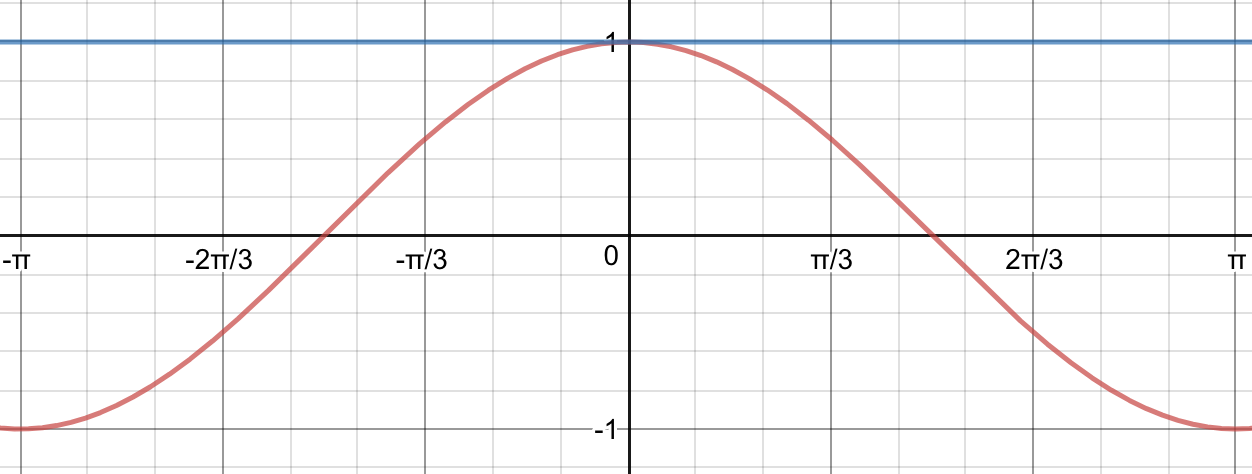
\includegraphics[width=0.5\textwidth]{taylor1st}
\end{figure}


\par{ This is far from a good approximation, but we have found one constant for our polynomial. Next we can think of other information we can get from $cos(x)$ near $x=0$. We know how to differentiate, hence he can get the rate of change of the function at $0$}

\item Finding the first order derivative for $f(x) \text{ and } g(x)$ we have that $f'(0) = -\sin(0) = 0$ and $g'(0) =  c_1 + 2c_2(0) + 3c_3(0)^2 + \dots = c_1$ . Again by equating the two derivatives we find that $c_1 = 0$. We now have: 

$$ g(x) = 1 + c_2x^2 + \cdots $$

\par{ Which did not help much, but we can still get more information, this time from the second-order derivative, and by repeating this process we'll get more and more terms for $g(x)$,and our approximation will be more and more accurate}

\item For up to the $6^{th}$ higher-order derivative we have that :

\begin{figure}[h]
\centering
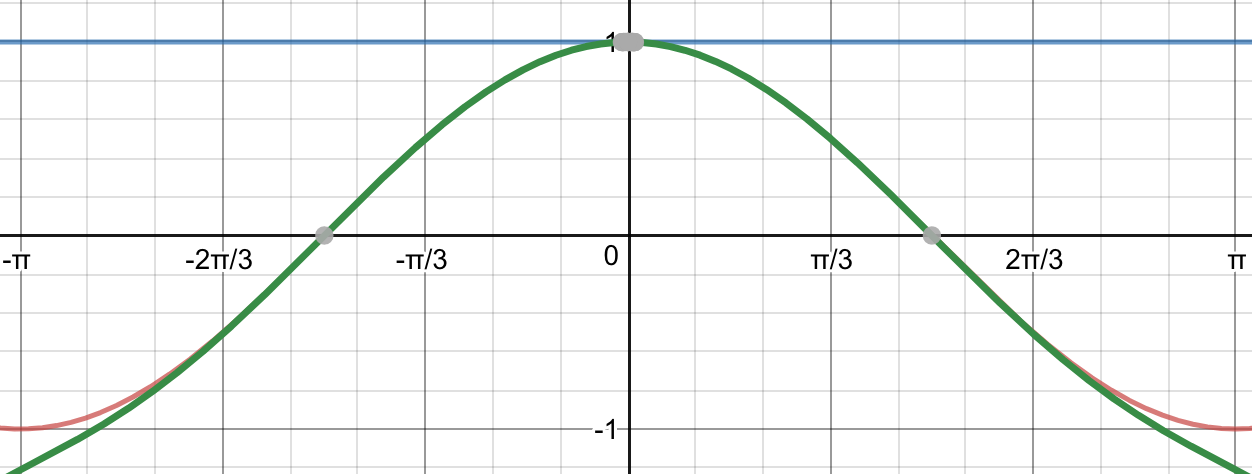
\includegraphics[width=0.5\textwidth]{taylor2nd}
\end{figure}


$$ g(x) = 1 + \frac{x^2}{2} + \frac{x^4}{24} + \frac{x^6}{720} $$

If we plugin a value into our polynomial, we find that the result is $\approx 98\%$ accurate comparing to the one obtained by a calculator. 

We still do not know "when to stop". For a periodic function like $\cos(x)$ this is sort of irrelevant, but for other functions which do not behave so regularly we can erroneously assume that our approximation is accurate anywhere in their domain, which in certain cases would be wrong \ref{taylor:rangeval}. How can we solve our \ita{infinite sum problem}

\item Lets first note that for each new term we generate, there seems to emerge a pattern. Every time we found a new higher order derivative , every other term we are not considering, remains unchanged *. \mymarginpar{*since they either differentiate to $0$ (l.o.t) or are multiplied by $0$ (h.o.t).} Furthermore, since $g(x)$ is a polynomial, every time we differentiate to find $c_n$ we find that the powers of \ita{h.o.t} accumulate, s.t. when we reach the $n^{th}$ term, the coefficient of $x$ is equal to n! which needs to be cancelled in order to obtain $c_n$, so the inverse is taken. So, at x = 0:

$$ c_n = \frac{1}{n!}f^{(n)}(0) \label{taylor:cN} $$

\nota{ $f'^{(n)}$: the $n^{th}$ order derivative}

\item \mymarginpar{*for example, the $18^{th}$ term of our example above yields 0.0000000002679245561}After coming to the conclusion above (\ref{taylor:cN}), we observe that if the series converges \ref{taylor:ratio} towards a limit, then as the \ita{h.o.t} become larger, they become less and less significant*. Let the first $n$ "significant" terms of the polynomial represent a \ita{truncated power series} \ref{taylor:powerSeries} \ref{taylor:taylorpoly} , and all higher order ones - $O(x^n)$ - or - $R_n(x)$ - be the \ita{remainder} of the series. Then if $ \lim_{n\to\infty}R_n(x) = 0$ , $f(x)$is just the sum of the series up until n.

\nota{$O(x^n)$ : All all the omitted terms are of $n^{th}$ order or higher in $x$}
\newpage
\subsection{Calculating}

\textbf{Putting it all together:}

\defn{Power Series\label{taylor:powerSeries} \ \ \ \ \ }{$ \sum _ { n = 0 } ^ { \infty } a _ { n } x ^ { n }$}

\defn{Taylor Series*\mymarginpar{*of $f$ at $a$}}{$$ \ \ \ \ \sum_{n=0}^{\infty}\frac{f^{(n)}(a)}{n!}(x-a)^n$$ \label{taylor:taylordef}}

\defn{Taylor Polynomial \label{taylor:taylorpoly}}{ A polynomial which higher order derivatives are designed to matchup with the original function (truncated Taylor series)}

\rem{Note that the example above evaluates the derivatives at $0$ because it is "cleaner" to do so, but we can start at any point where the value of the function is known. When starting at $0$ the series are called \textbf{McLaurin Series} \ref{taylor:mc} }

\defn{McLaurin Series \label{taylor:mc}}{$$ \ \ \ \ \sum_{n=0}^{\infty}\frac{f^{(n)}(0)}{n!}(x)^n$$}

\defn{Range of Validity\label{taylor:rangeval}}{ The values of $x$ for which the infinite sum exists and is equal to $f(x)$} \mymarginpar{TO DO: Method for finding it}
 
\end{enumerate}

 \extra{The Ratio Test \label{taylor:ratio} \begin{enumerate}
\item Convergent if $\lim_{n\to\infty} = \Big|\frac{a_{n+1}}{a_n}\Big| < 1$
\item Divergent if $ \lim_{n\to\infty} = \Big|\frac{a_{n+1}}{a_n}\Big| > 1$
\item Inconclusive if $ \lim_{n\to\infty} = \Big|\frac{a_{n+1}}{a_n}\Big| = 1$
\end{enumerate}}

\newpage
\lecture{11}{01}{2019}

\subsection{Important Series}

$$e ^ { x } = 1 + \frac { x } { 1 ! } + \frac { x ^ { 2 } } { 2 ! } + \frac { x ^ { 3 } } { 3 ! } + \frac { x ^ { 4 } } { 4 ! } + \cdots \quad x \in \mathbb { R }$$

$$\sin x = x - \frac { x ^ { 3 } } { 3 ! } + \frac { x ^ { 5 } } { 5 ! } - \frac { x ^ { 7 } } { 7 ! } + \cdots \quad x \in \mathbb { R }$$

$$\cos x = 1 - \frac { x ^ { 2 } } { 2 ! } + \frac { x ^ { 4 } } { 4 ! } - \frac { x ^ { 6 } } { 6 ! } + \cdots \quad x \in \mathbb { R }$$

$$\log ( 1 + x ) = x - \frac { x ^ { 2 } } { 2 } + \frac { x ^ { 3 } } { 3 } - \frac { x ^ { 4 } } { 4 } + \frac { x ^ { 5 } } { 5 } - \cdots \quad x \in ( - 1,1 ]$$

$$( 1 + x ) ^ { \lambda } = 1 + \left( \begin{array} { c } { \lambda } \\ { 1 } \end{array} \right) x + \left( \begin{array} { c } { \lambda } \\ { 2 } \end{array} \right) x ^ { 2 } + \left( \begin{array} { c } { \lambda } \\ { 3 } \end{array} \right) x ^ { 3 } + \cdots \quad x \in \left\{ \begin{array} { c c } { ( - 1,1 ) } & { \text { if } \lambda < 0 } \\ { \mathbb { R } } & { \text { if } \lambda \geqslant 0 } \end{array} \right.$$


\ex{Find the MacLaurin Series for $f(x) = e^x$}

\par{We start by noting that $f^{(n)}(x) = e^x$ . Hence evaluating it at $ x = 0 $, we get $f^{(n)}(o) = e^0 = 1$. Therefore we can find the constant terms of the series by applying \ref{taylor:cN}, giving us:}

$$ c_n = \frac{1}{n!}$$

and so,

$$ e^x = \sum^{\infty}_{n=0}\frac{x^n}{n!} = 1 + \frac{x}{1!} + \frac{x^2}{2!} + \frac{x^3}{3!} + \dots$$

\ex{Find the Maclaurin Series for $g(x) = \log(1+x)$}

\begin{enumerate}
	\item We'll start by substituting $(1+x)$ so that we can observe the behaviour of the more general logarithm.
	
	Let $1 + x = y$ , then we have the common $\log$ derivative, $g(y)'=(\log(y))' = \tfrac{1}{y}$. What of the $n^{th}$ derivative? By differentiating the next 3 terms we notice a pattern emerging:
	
	\begin{align*}
		&g''(y) = -y^{-2} \\
		&g'''(y) = 2y^{-3} \\
		&g^{iv}(y) = 2(-3)y^{-4}
	\end{align*}
	
Therefore we have:

$$ g^{(n)}(y) = (-1)^{n-1}(n-1)!y^{-n} $$

	\item Hence, by application of the chain rule we get:
	
	$$ g^{(n)}(x) = \frac{d^{(n)}}{dy} log(y) \times \frac{d}{dx} (1 + x) =  \frac{(-1)^{n-1}(n-1)!y^{-n}}{1} = \frac{(-1)^{n-1}(n-1)!}{(1+x)^n}$$
	
	\item Evaluating it at $x = 0$, gives us the following first 4 terms: $ 0 , 1 , -\frac{1}{2} , \frac{1}{3}$
\end{enumerate}

\par{So that we have the approximation being given by the series: $$x - \frac{x^2}{2} + \frac{x^3}{3}  + \dots$$}

\lecture{17}{01}{2019}
\subsection{Manipulation of Series}

\begin{enumerate}

	\item \textbf{Addition}
		$$f(x) + g(x) = \sum_{n=0}^{\infty}(f_n+ g_n) x^n$$
	
	\item \textbf{Multiplication}
		$$\begin{aligned} f ( x ) g ( x ) & = \left( \sum _ { n = 0 } ^ { \infty } f _ { n } x ^ { n } \right) \left( \sum _ { m = 0 } ^ { \infty } g _ { m } x ^ { m } \right) \\ & = \sum _ { n = 0 } ^ { \infty } \left( \sum _ { r = 0 } ^ { n } f _ { r } g _ { n - r } \right) x ^ { n } \end{aligned}$$
		
		\ex{$f(x) = \frac { e ^ { 2 x } } { 1 - x }$ first 3 terms of the McLaurin series}
		
		\par{First we note that the function can be seen as the multiplication of two separate functions $g(x) = e^{2x}$ and $h(x) = (1-x)^{-1}$. Since we know the series for $e^y$, let y = 2x so that we have:}
		\begin{align*}
		e^ y &= 1 + \frac { y } { 1 ! } + \frac { y ^ { 2 } } { 2 ! } + \frac { y ^ { 3 } } { 3 ! } + \frac { y ^ { 4 } } { 4 ! } + \cdots , \quad y \in \mathbb { R } \\
	& = 1 + 2 x + 2 x ^ { 2 } + \frac { 4 x ^ { 3 } } { 3 } + \frac { 2 x ^ { 4 } } { 3 } + \cdots , \quad x \in \mathbb { R }
	\end{align*}
			
	\begin{align*}(1-x)^{(-1)} = 1 + x + x^2 + x^3 + x^4 + \cdots\end{align*}
	
	\par{Hence,}
	
	$$(e^2x) (1-x)^{(-1)} = (1 + 2 x + 2 x ^ { 2 } + \frac { 4 x ^ { 3 } } { 3 } + \frac { 2 x ^ { 4 } } { 3 } + \cdots) (1 + x + x^2 + x^3 + x^4 + \cdots) $$
	
	\par{Now we inspect which terms, when multiplied, will result in degree 3 or less and ignore the \ita{h.o.t}. So that we have:}
	
	$$ (e^2x) (1-x)^{(-1)} = 1 + 3 x + 5 x ^ { 2 } + \frac { 19 } { 3 } x ^ { 3 } + O(x^4) $$
	
	\item \textbf{Functions' Composition}
	
	$$f ( g ( x ) ) = \sum _ { n = 0 } ^ { \infty } f _ { n } \left( \sum _ { m = 0 } ^ { \infty } g _ { m } x ^ { m } \right) ^ { n }$$
	
	\ex{$\log ( \cos x ) \text { up to the term } x ^ { 6 }$}
	
	\par{Again, the underlining idea is to try and rewrite the expression so that we can use one of the simpler, known series.}
	
	$$ \log ( \cos x ) = \log \left( 1 + \boxed{( - 1 + \cos x )} \right) = \log ( 1 + y ) $$
	
	\par{Now it's possible to use the series for $ \log(1+x)$ that we've seen above.}
	
	$$ \log ( 1 + y ) = y - \frac{y^2}{2} + \frac{y^3}{3} + O(x^4) $$
	
	\par{ Note however, that $y$ must still satisfy the range of validity for the $\log$ function. Hence,}
	
	$$- 1 \leqslant - 1 + \cos x \leqslant 1 \iff 0 \leqslant \cos x \leqslant 2 $$
	
	\par{Finding the series for the inner function $1-\cos(x)$, gives us:}
	
	$$\begin{aligned} - 1 + \cos x & = \cancel{- 1} +  \left( \cancel{1} - \frac { x ^ { 2 } } { 2 ! } + \frac { x ^ { 4 } } { 4 ! } - \frac { x ^ { 6 } } { 6 ! } + O(x^7) \right) \\ & = - \frac { x ^ { 2 } } { 2 ! } + \frac { x ^ { 4 } } { 4 ! } - \frac { x ^ { 6 } } { 6 ! } - O(x^7) \end{aligned}$$
	
	\par{Finally, let $g(x) = 1- \cos(x)$ and $f(x) = \log(1+y)$ substituting $g(x)$ back into the series of $f(x)$ by application of the formula for composite series. We have,}
	
	$$\begin{aligned}
		\log\left(\cos(x)\right) &= y - \frac { 1 } { 2 } y ^ { 2 } + \frac { 1 } { 3 } y ^ { 3 } - \frac { 1 } { 4 } y ^ { 4 } + \cdots \\
			&= \left( - \frac { x ^ { 2 } } { 2 ! } + \frac { x ^ { 4 } } { 4 ! } - \frac { x ^ { 6 } } { 6 ! } - \cdots \right) - \frac { 1 } { 2 } \left( - - \frac { x ^ { 2 } } { 2 ! } + \frac { x ^ { 4 } } { 4 ! } - \frac { x ^ { 6 } } { 6 !} + \cdots \right) ^ { 2 } +  \\ & \ \frac { 1 } { 3 } \left( - \frac { x ^ { 2 } } { 2 ! } + \frac { x ^ { 4 } } { 4 ! } - \frac { x ^ { 6 } } { 6 !} + \cdots \right) ^ { 3 } + \cdots \\
			&= - \frac { x ^ { 2 } } { 2 } - \frac { x ^ { 4 } } { 12 } - \frac { x ^ { 6 } } { 45 } + O(x^7)
			\end{aligned}$$

\end{enumerate}

\lecture{18}{01}{2019}

\mymarginpar{TODO: Error using remainder, limits, complex arguments}

\section{Integration}

\lecture{24}{01}{2019}

\subsection{The Area Under The Curve}

\par{The \textbf{key idea} of this section is to understand that we can \ita{approximate} the area of non-regular shapes, like curves, by inscribing (or out-scribing) a regular polygon of which we can easily calculate the area of}

\rem{It is self-evident that the more polygons we use, the closer we get to completely cover the area under the curve.~\label{area:accurate}}

\rem{Following from (\ref{area:accurate}) , it is also clear that by using the notion of limit  (just like we saw in the chapter before) we should expect the total area to tend towards a number, i.e. by using a very large number of polygons (as $n \to \infty$) the overall area covered is equal to that of the curve}

\ex{Estimating the area under the curve $f(x) = x^2$ between 0 and 1}

\par{Let's start by comparing the estimates when using 4 and 16 rectangles with their left edges touching the curve.}

\begin{enumerate}
	\item{Calculating the width of the rectangles: We need to split the interval given $[0,1]$ into 4 and 16 equal parts. Let $\delta x$ represent the width for the 4-way split, and $delta y$ the 16-way split.}
	
	$$\delta x = \frac{1-0}{4} = \frac{1}{4} \quad \quad \delta y = \frac{1-0}{16} = \frac{1}{16}$$
	
	\item{Calculating the heights for each rectangle: Note that to calculate the height, all we need to do is to evaluate $f(x)$ where the rectangle and it meet. Since we've decided to draw the first rectangle starting its left-edge from $0$ and given that they'll have fixed width, we find that the height for a general $n^{th}$ rectangle is given by $0 + (n-1) (\frac{1}{4})$. Such that:
	
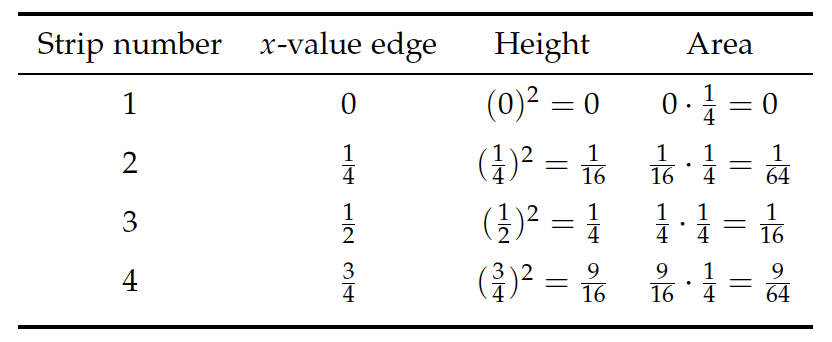
\includegraphics[width=15em]{area4strips}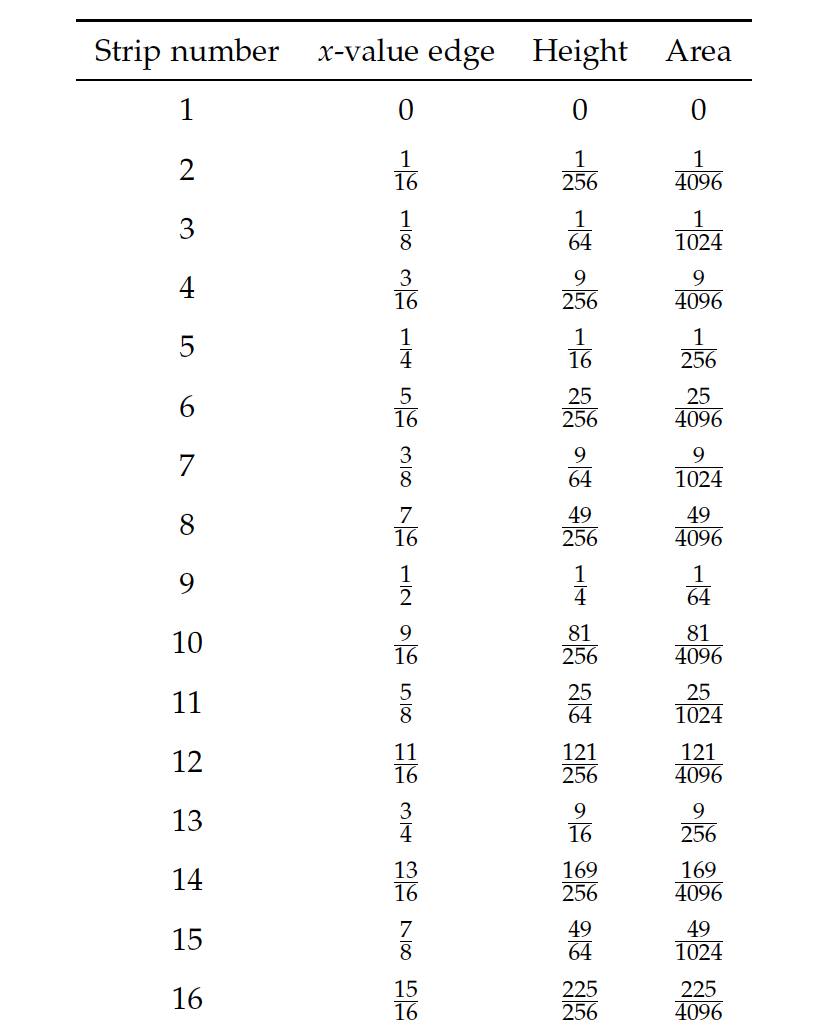
\includegraphics[width=15em]{area16strips}
}

	\item{Summing the areas $(R_n)$ of the rectangles to get an approximation of the area under the curve, we get:
	
	$$R_4 = 0.21875 \quad \quad R_16 = 0.302734375 $$
	
	
	}
	

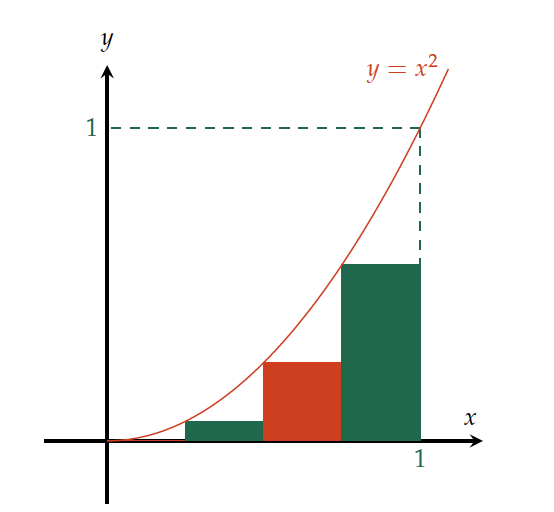
\includegraphics[width=15em]{area4strips2} 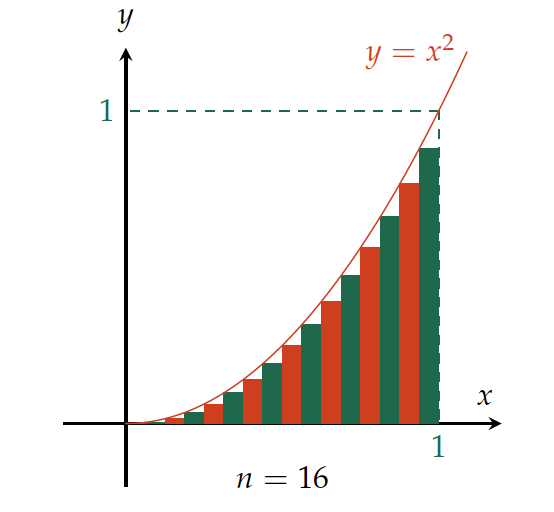
\includegraphics[width=15em]{area16strips2}
	
\end{enumerate}

\par{Note as remarked above, that by increasing the number of rectangles the area under the curve not accounted for decreases, therefore the approximation becomes more accurate. In fact, we can see that by very large numbers the area will tend towards $\tfrac{1}{3}$, giving us the precise area}

\rem{We chose to draw the rectangles matching their left edges with points in the curve, but we could equally have chosen the right edge or the middle point. The difference between the accuracy of the left and right edge approach depends of the shape of the curve. Choosing the middle point will however, always give us the best estimate, since it overestimates from one side, but it "compensates" by underestimating on the other. See (\ref{Riemann:middle}) for a detailed illustration}

\newpage
\subsection{Calculating the Area by Evaluating the Limit of $R_n$}

\par{We can use our knowledge of series from 1R and from the previous chapter to evaluate the sum of a very large number of polygons, to get an exact value of the area under the curve}

\ex{Show that $\lim_{n \to \infty} R_n = \frac{1}{3}$

\par{By using a k number of strips, we have that their width is given by $\frac{1}{k}$, and the left edge value of the $j^{th}$ strip is then given by $0+(\frac{j}{k})^2$ or simply $(\frac{j}{k})^2$ since we are starting at $ x = 0 $. Finally the area of each strip is given by $\frac{1}{k} \cdot (\frac{j}{k})^2$ and their sum $(R_k)$:}

$$R_k = 0 + \frac{1}{k^2} + \left(\frac{2}{k}\right)^2 + \dots + \left(\frac{k-1}{k}\right)^2 = \frac{1}{k^3} \sum_{j=1}^{k-1}j^2$$

\rem{Remember the \textbf{sum of squares} \scriptsize{see algebra \ita{5.6}} \normalsize: $$\sum_{l=1}^{n} l^2 = \frac{n(n+1)(2n+1)}{6}$$}
}

\par{Hence:}

\begin{align*}
 R_k &= \frac{1}{k^3} \sum_{j=1}^{k-1} (k-1)^2 \\ 
 &= \frac{(k-1)((k-1)+1)(2(k-1)+1)}{6} \\
 &= \frac{2k^3 - k^2 - 2k^2 + k}{6k^3} \\
 &= \frac{1}{3} - \frac{1}{2k} + \frac{1}{6k^2}
 \end{align*}
 
 \par{So, as $n \to \infty$:}
 
 $$R_k = \frac{1}{3} - \underbrace{\frac{1}{\infty}}_0 + \underbrace{\frac{1}{\infty}}_0 = \frac{1}{3}$$
 
 \par{In general then, we have:}
 
 \defn{Area under the curve ~\label{area:limit}}{Let $y = f (x)$ be a continuous function and $a, b$ two values in the domain of $f$ . Then the area under the curve $y = f (x)$
between $x = a $and $x = b$ is the limit of the sum of the areas of the
rectangular strips:
 
 $$\lim_{n \to \infty}\sum_{j=0}^{n-1}f(x_j)\delta x$$}
 
 \newpage
 
 \subsection{Definite Integral}
 
 \defn{Definite Integral}{The limit of the sum of the areas of the rectangular strips (\ref{area:limit}) as the number of strips tend to infinity. $A$ is the integral from $ x = a $ to $x = b$ of $f(x)$ with respect to $x$ 
 $$ A = \int_{a}^{b} f(x) dx$$}
 
 \defn{Limits of Integration}{The interval $[a,b]$}
 
 \subsection{Riemann Sum Estimates}
 
 \par{Putting the 2 previous concepts together, we have the concept of \ita{Riemann Sums}}
 
 \defn{Riemann Sum}{An approximation to the area under the graph given by the sum of the areas of $n$ rectangles. Let $\delta x = \frac{b-a}{n}$ represent the width of each rectangle and $x_j = a + j\delta x$ represent the points where they meet the curve. Then, the area is given by:
 
 $$ \lim_{\delta x \to 0} \left(\sum_{j=0}^{j=n-1}f(x_j)\delta x\right) = \lim_{n \to \infty} \left(\sum_{j=0}^{j=n-1}f(x_j)\delta x\right) $$}
 
\ex{
\par{Given $f(x) = x^3 - x$ , find its Riemann sum between $[0,2]$ and its definite integral}


}
\newpage
\nocite{*}
\printbibliography

\end{document}

